\documentclass[aspectratio=169]{beamer}
\mode<presentation>

%Theme and Color of Presentation
\usetheme{CambridgeUS}
\usecolortheme{seahorse}
\useinnertheme{rectangles}

%Colors
% From https://www.utdallas.edu/brand/color-palette/
\definecolor{UTDorange}{RGB}{232,117,0}
\definecolor{UTDgreen}{RGB}{18,71,52}
\definecolor{UTDseafoam}{RGB}{95,244,183}

\setbeamercolor{palette primary}{bg=UTDorange,fg=white}
\setbeamercolor{palette secondary}{bg=UTDgreen,fg=white}
\setbeamercolor{palette tertiary}{bg=UTDorange,fg=white}
\setbeamercolor{palette quaternary}{bg=UTDorange,fg=white}
\setbeamercolor{frametitle}{fg=UTDgreen}
\setbeamercolor{structure}{fg=UTDgreen} % itemize, enumerate, etc
\setbeamercolor{subsection in head/foot}{bg=UTDgreen,fg=white}


%Additional Packages
\usepackage{graphicx}
% \usepackage{svg}
\usepackage{physics}
\usepackage{setspace}
\usepackage{textpos}

%Additional Settings/Commands
\newcommand{\extraspace}{\vskip 0.5em}

\AtBeginSection[]
{
	\begin{frame}
		\frametitle{Outline}
		\tableofcontents[currentsection]
	\end{frame}
}
%\AtBeginSubsection[]
%{
%	\begin{frame}
%		\frametitle{Outline}
%		\tableofcontents[currentsection,currentsubsection]
%	\end{frame}
%}

%Presentation Info
\title[]{Path Planning for Autonomous Vehicles based on Nonlinear MPC with using a Kinematic Bicycle Model}
\subtitle{}
\author{Jonas Wagner}
%\institute[UTDallas]{Univeristy of Texas at Dallas}
\date[MECH 6V29 MPC - Fall 2023]{MECH 6V29 - MPC\\ Fall 2023}


\begin{document}
	
\begin{frame}
	\titlepage
\end{frame}

\addtobeamertemplate{frametitle}{}{%
	\begin{textblock*}{100mm}(.85\textwidth,-1cm)
		
\includegraphics[height=1cm]{figs/UT_Dallas_Logo}
	\end{textblock*}
}

\begin{frame}{Outline}
	\tableofcontents
\end{frame}

\section{System Overview}
% \subsection{Hail Bopp}
\begin{frame}
	\frametitle{NOVA: Hail Bopp \cite{nova}}
	\begin{columns}
		\begin{column}{0.25\textwidth}
			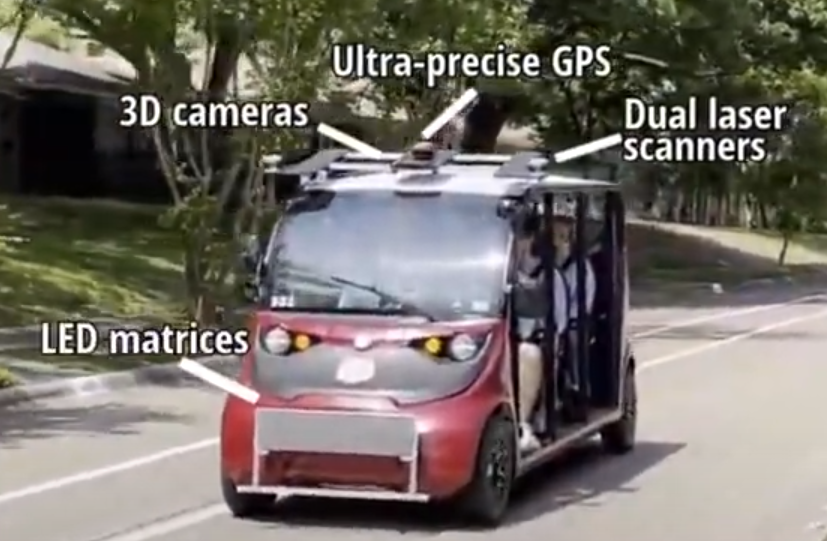
\includegraphics[width=\columnwidth]{figs/NOVA-annotatedImage.png}
		\end{column}
		\begin{column}{0.3\textwidth}
			
\includegraphics[width=\columnwidth]{figs/NOVA-logo.png}
		\end{column}
	\end{columns}
\end{frame}
\begin{frame}
	\frametitle{NOVA: Perception \cite{nova}}
	\begin{columns}
		\begin{column}{0.7\textwidth}
			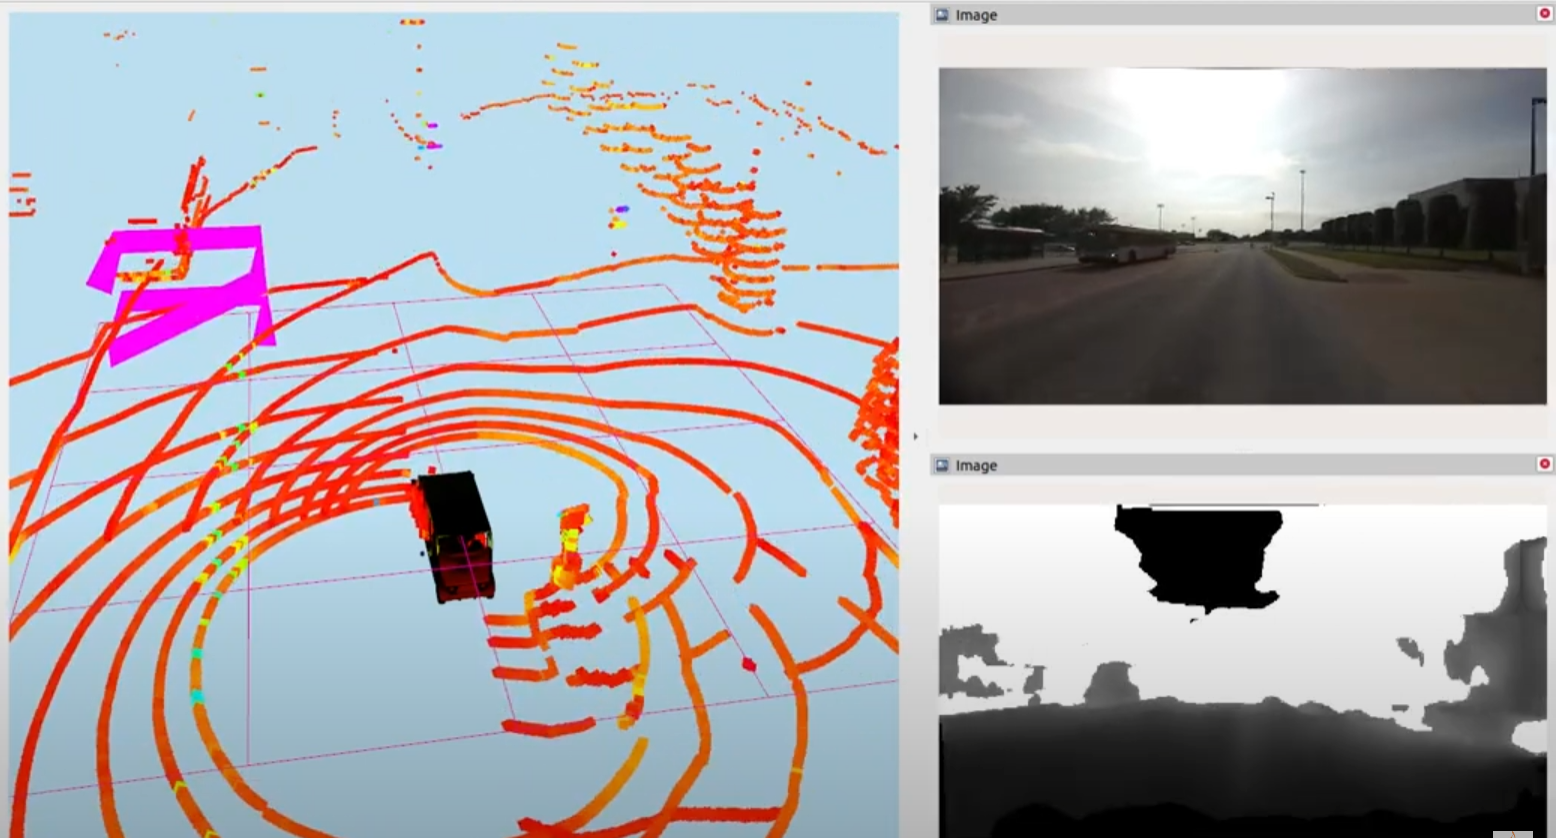
\includegraphics[width = \columnwidth]{figs/NOVA-sensorData_screenshot.png}
		\end{column}
	\end{columns}
\end{frame}

% \subsection{Navigator}
\begin{frame}
	\frametitle{NOVA: Navigator \cite{nova}}
	\begin{columns}
		\begin{column}{0.6\textwidth}
			\begin{itemize}
				\item Navigator is the self-driving software stack being developed by NOVA.
				\item Simulations done in then deployed to Hail Bopp.
			\end{itemize}
		\end{column}
		\begin{column}{0.4\textwidth}
			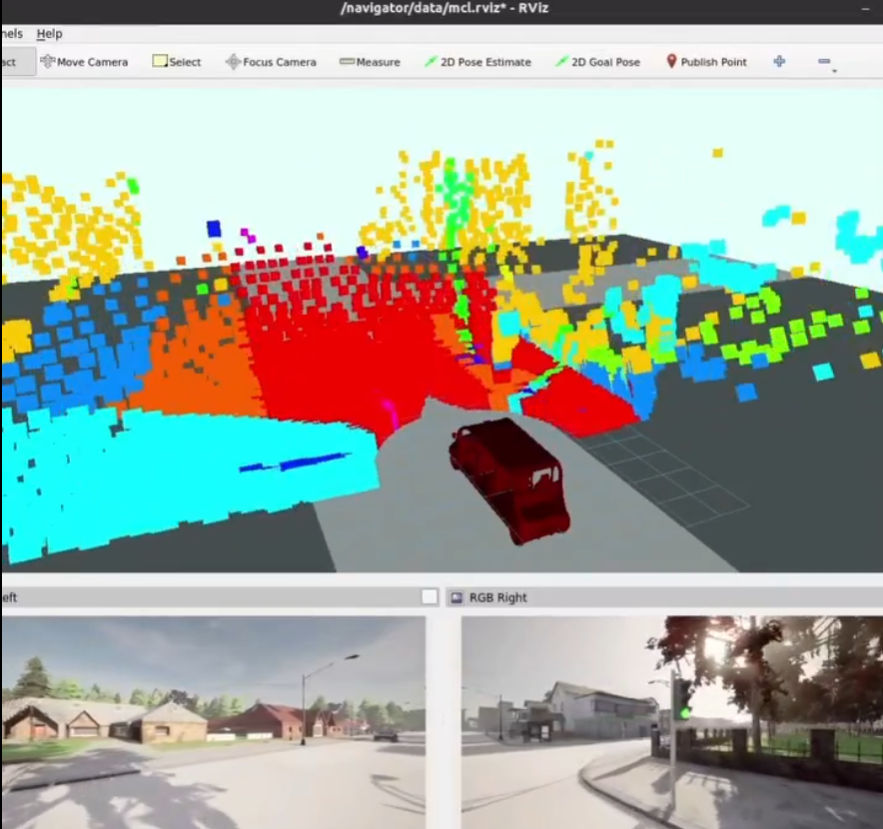
\includegraphics[width = \columnwidth]{figs/NOVA-carla_screenshot.png}
		\end{column}
	\end{columns}
\end{frame}

\begin{frame}
	\frametitle{Path Planning Objective \cite{nova}}
	Current Approach (random path generation and ranking)
	\begin{columns}
		\begin{column}{0.3\textwidth}
			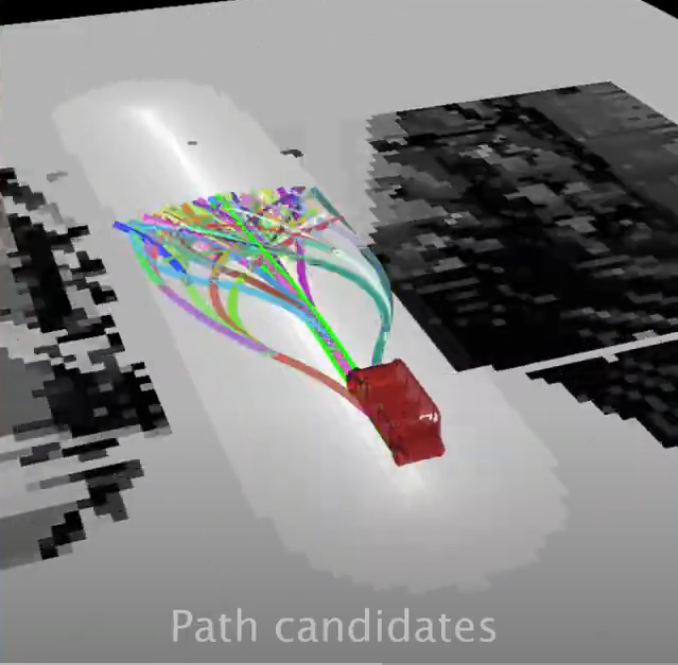
\includegraphics[width = \columnwidth]{figs/NOVA-demo2_pathCanidates.png}
		\end{column}
		\begin{column}{0.35\textwidth}
			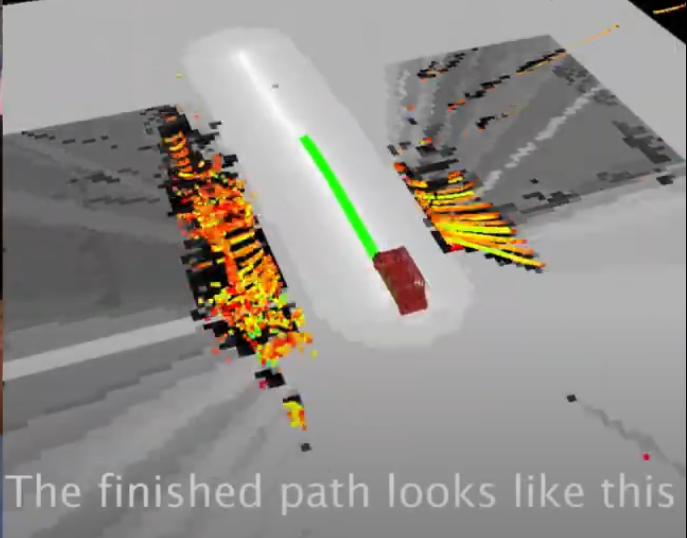
\includegraphics[width = \columnwidth]{figs/NOVA-demo2_pathSolution.png}
		\end{column}
	\end{columns}

	\textbf{Objective:} 
	Develop NL-MPC based path planning that is better than the current aproach.

	(Spoiler: NL-MPC is too complicated for this portion of Navigator's stack at this stage and many more efficient techniques exist.
	MPC will become more benificial when robustness/security gaurentees are required/desired).
\end{frame}

\section{System Model}
% \subsection{Vehicle Modeling}

\begin{frame}
	\frametitle{Vehicle Kinematic Models \cite{casanova_thesis,vehcileDynamics_chapter2a}}
	\begin{columns}
		\begin{column}[t]{0.6\textwidth}
			Akerman Steering Model
			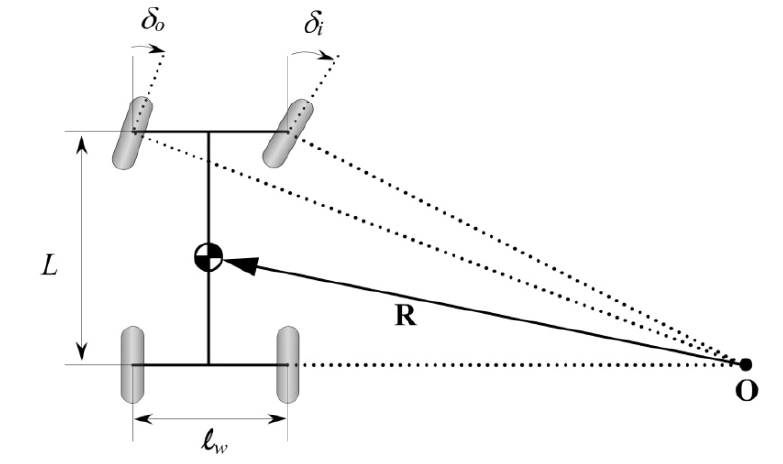
\includegraphics[width = 0.7\columnwidth]{figs/akermanModel.png}

			Akerman steering can be approximated as a bicycle model in most cases.
		\end{column}
		\begin{column}[t]{0.3\textwidth}
			Bicycle Approximation
			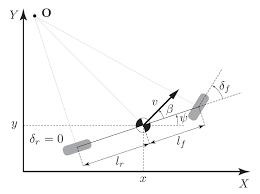
\includegraphics[width = \columnwidth]{figs/bikeModel.png}
			\[\delta \approx \cfrac{\delta_o + \delta_i}{2}\]
		\end{column}
	\end{columns}

\end{frame}
% \subsection{Bicycle Model}

\begin{frame}
	\frametitle{Kinematic Bicycle Model \cite{Rajamani2012}}

	\begin{columns}
		\begin{column}{0.4\textwidth}
			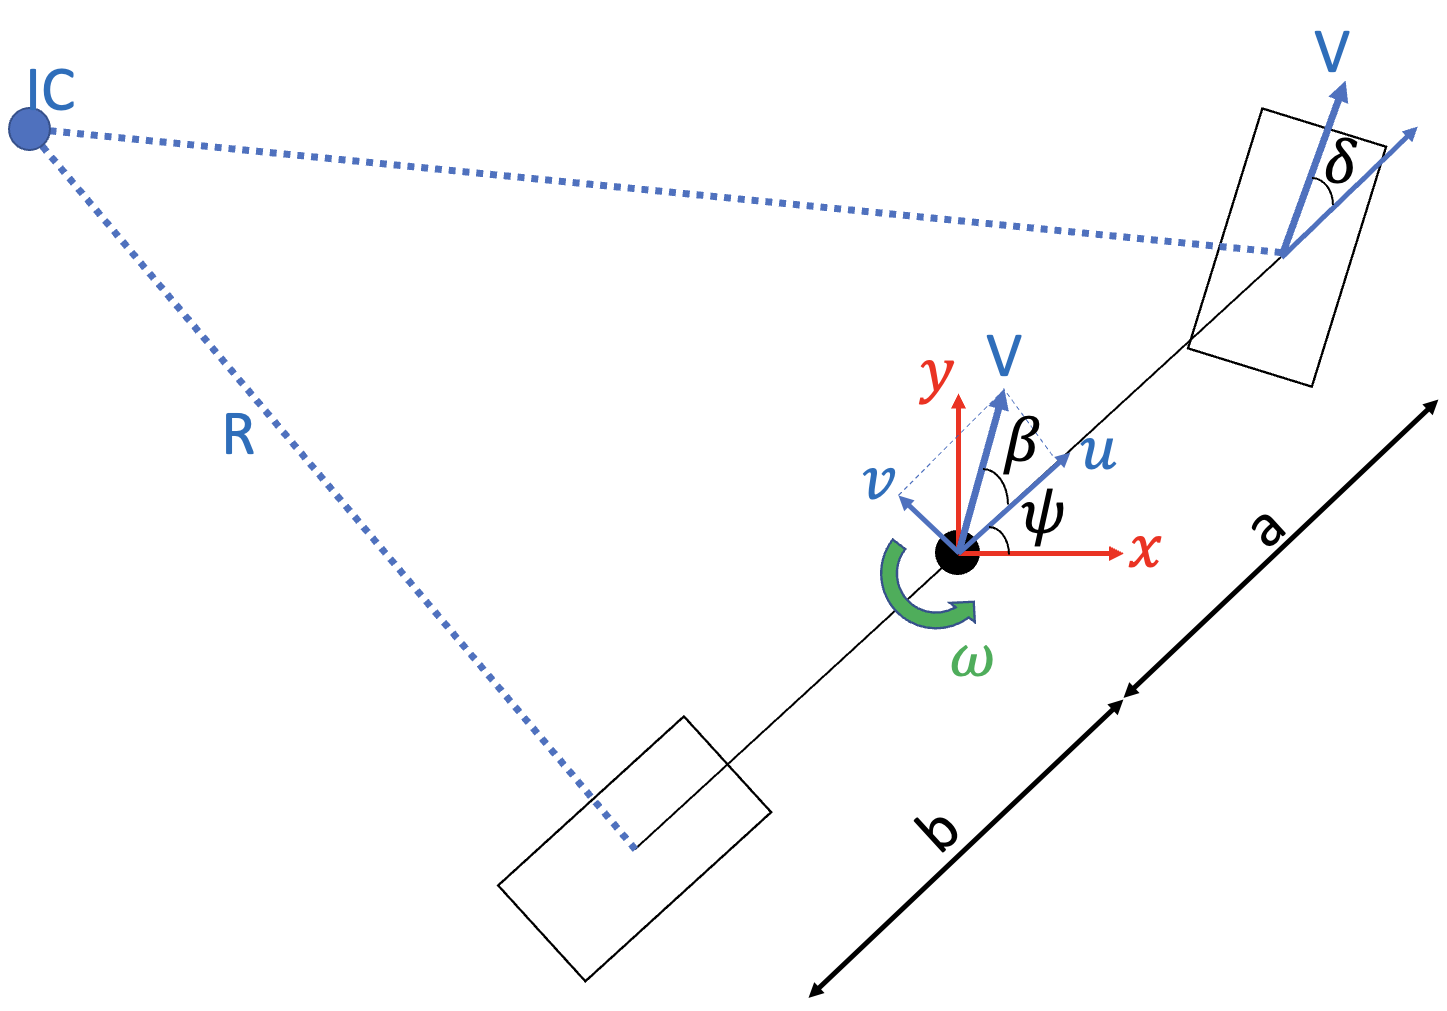
\includegraphics[width=\columnwidth]{figs/BicycleModel.png}
		\end{column}
		\begin{column}{0.5\textwidth}
			Simple nonlinear kinematics model equations:
			\begin{equation}
				\begin{cases}
					\dot{x} = V \cos(\psi + \beta)\\
					\dot{y} = V \sin(\psi + \beta)\\
					\dot{\psi} = \cfrac{V \cos(\beta)}{l_f + l_r} \qty(\tan(\delta_f) - \tan(\delta_r))\\
					\dot{\theta} = \psi
				\end{cases}
			\end{equation}
			where
			\begin{equation}
				\beta = \tan^{-1}\qty(\cfrac{l_f \tan(\delta_r) + l_r \tan(\delta_f)}{l_f + l_r})
			\end{equation}
			$\delta_r = 0$, $l_f = a = 0.7 [m]$, and $l_r = b = 0.7 [m]$.
		\end{column}
	\end{columns}

\end{frame}

\section{Nonlinear MPC Formulation}
\begin{frame}
	\frametitle{Model Discretization\cite{rk4}}
	\begin{columns}
		\begin{column}{0.6\textwidth}
			Discretized with $\Delta t = 1$ [s] using \textbf{RK4 method} 
			(euler method doesn't work without very small $\Delta t$) 
		\end{column}
		\begin{column}{0.4\textwidth}
			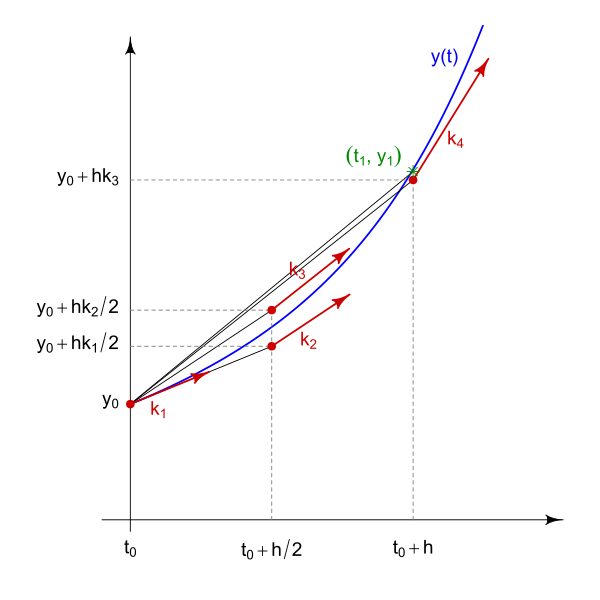
\includegraphics[width=\columnwidth]{figs/rk4_method.png}
		\end{column}
	\end{columns}
\end{frame}

\begin{frame}
	\frametitle{Input Constraints}
	\begin{columns}
		\begin{column}{0.5\textwidth}
			$V \in [0,10]$ [m/s]

			$\theta \in \pm \pi/3$ [rad]

			$\dot{V} \in [-4,2]$ [m/s\^2]

			$\dot{\theta} \in \pm \pi/10$ [rad/s]
		\end{column}
		\begin{column}{0.5\textwidth}
			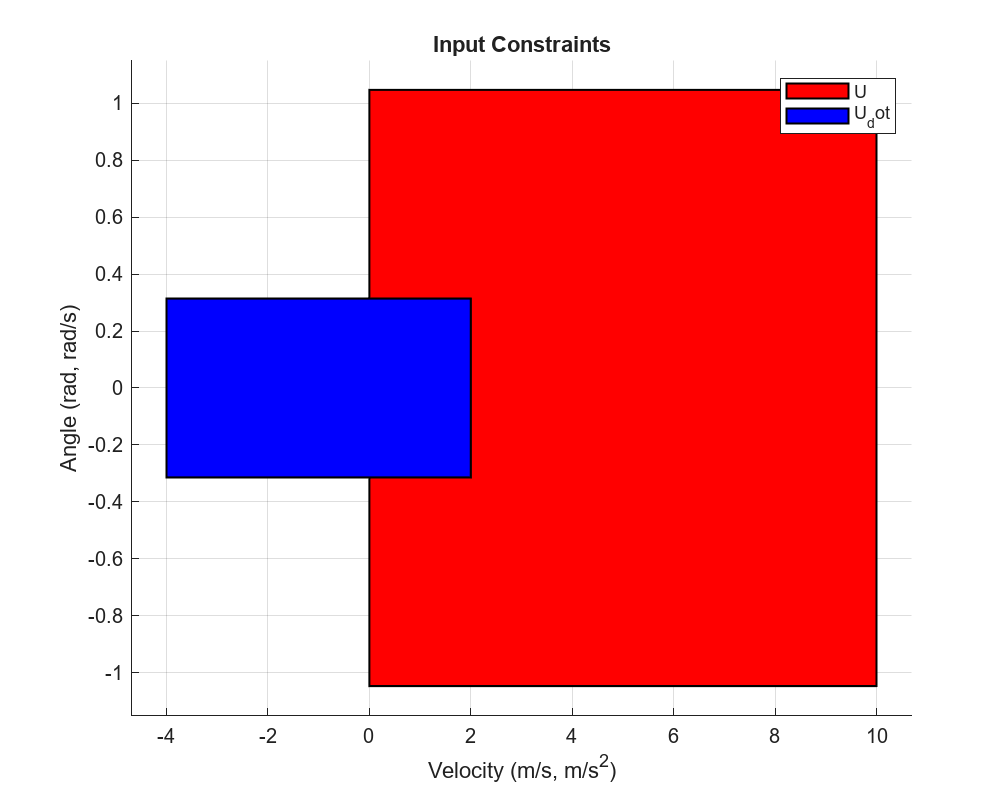
\includegraphics[width=\columnwidth]{figs/input_constraints.png}
		\end{column}
	\end{columns}
\end{frame}

\begin{frame}
	\frametitle{MPC Optimization Problem}

	\begin{columns}
		\begin{column}{0.5\textwidth}
			Parameters:
			\begin{itemize}
				\item $N = 15$
				\item $\Delta t = 1$ [s]
				\item Multiple $q(x_k,u_k)$ and $p(x_{n})$ tested
				\item $h(x_k,u_k) \ | \ u_k \in \mathbf{U} \land \dot{u}_k \in \dot{\mathbf{U}}$
				\item (for closed-loop sim: $T = 10$ [s])
			\end{itemize}
		\end{column}
		\begin{column}{0.5\textwidth}
			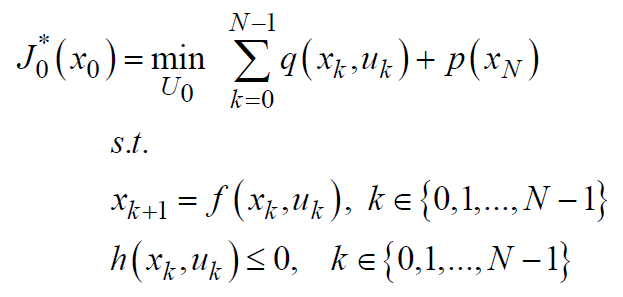
\includegraphics[width=\columnwidth]{figs/nl_mpc_equations.png}
		\end{column}
	\end{columns}

\end{frame}


%% Simulation Implementation and Results
\section{Simulation Implementation and Results}
% \subsection{Solver Selection}
\begin{frame}
	\frametitle{fmincon vs ipopt (Computation Time)}

	The results and computation time are GREATLY affected by the selection of the nonlinear optimization solver used.

	The following is a simple comparison of computation time (just for demonstration... not a controlled case study)
	
	\begin{table}[]
		\begin{tabular}{|l|l|l|}
		\hline
		\textbf{}                       & \textbf{FMINCON} & \textbf{IPOPT}  \\ \hline
		Min Y - Unstructured            & 243.79           & 164.75          \\ \hline
		Min Y - Final                   & 235.91           & 155.6           \\ \hline
		Min Y - Ref X and theta         & 438.67           & 71.79           \\ \hline
		\textbf{Min X - Final}          & \textbf{1077.6}  & \textbf{164.58} \\ \hline
		Min X with +180                 & 395.71           & 191.69          \\ \hline
		\textbf{Min X with special ref} & \textbf{344.52}  & \textbf{165.16} \\ \hline
		\textbf{Max Y - Final}          & \textbf{331.71}  & \textbf{140.49} \\ \hline
		\textbf{Max Y - Ref X theta}    & \textbf{665.82}  & \textbf{85.492} \\ \hline
		\end{tabular}
		\end{table}

\end{frame}


\begin{frame}
	\frametitle{fmincon vs ipopt (Min X w/ Final - Both Fail)}
	$J = x_{N+1}$
	\begin{columns}
		\begin{column}{0.4\textwidth}
			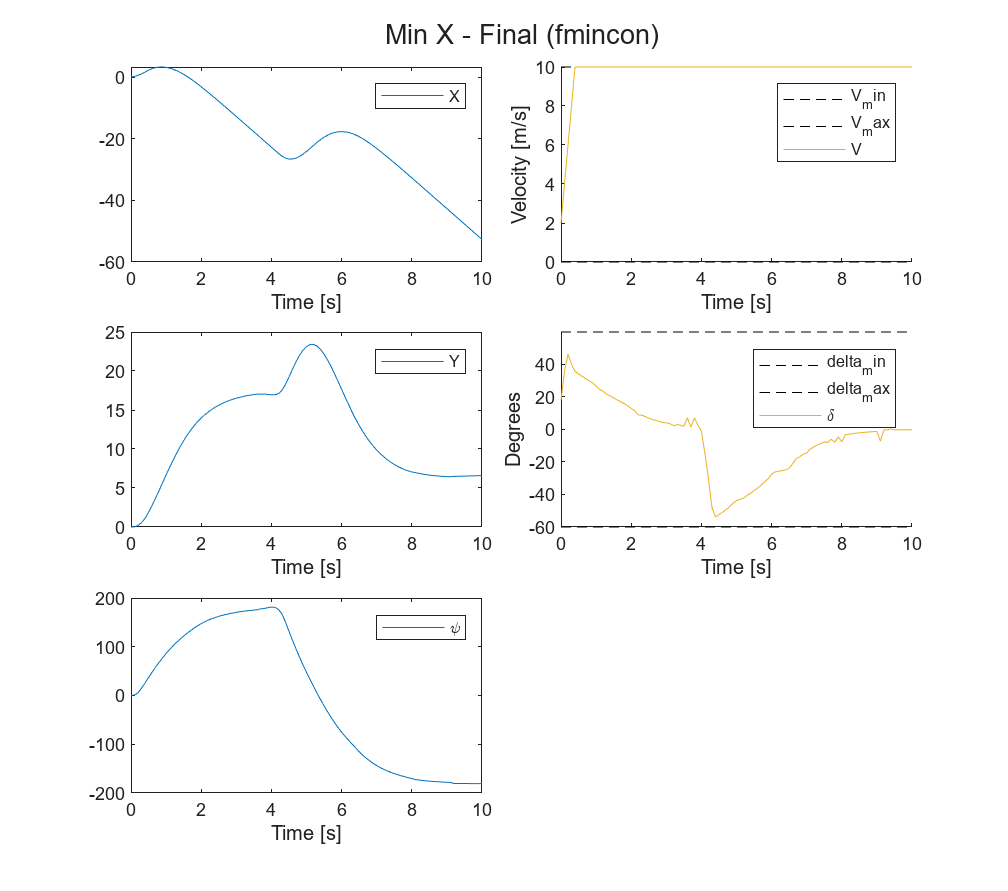
\includegraphics[width = \columnwidth]{figs/Min_X_-_Final_(fmincon)_traj.png}
		\end{column}
		\begin{column}{0.25\textwidth}
			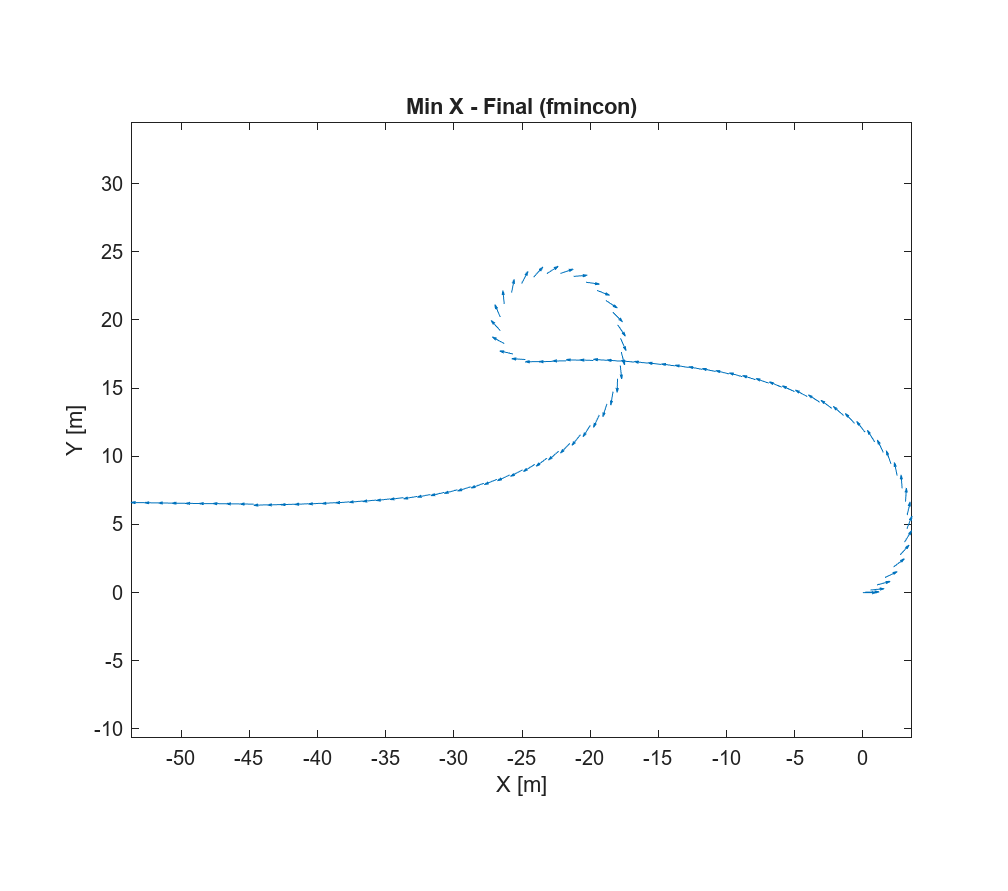
\includegraphics[width = \columnwidth]{figs/Min_X_-_Final_(fmincon)_quiver.png}
			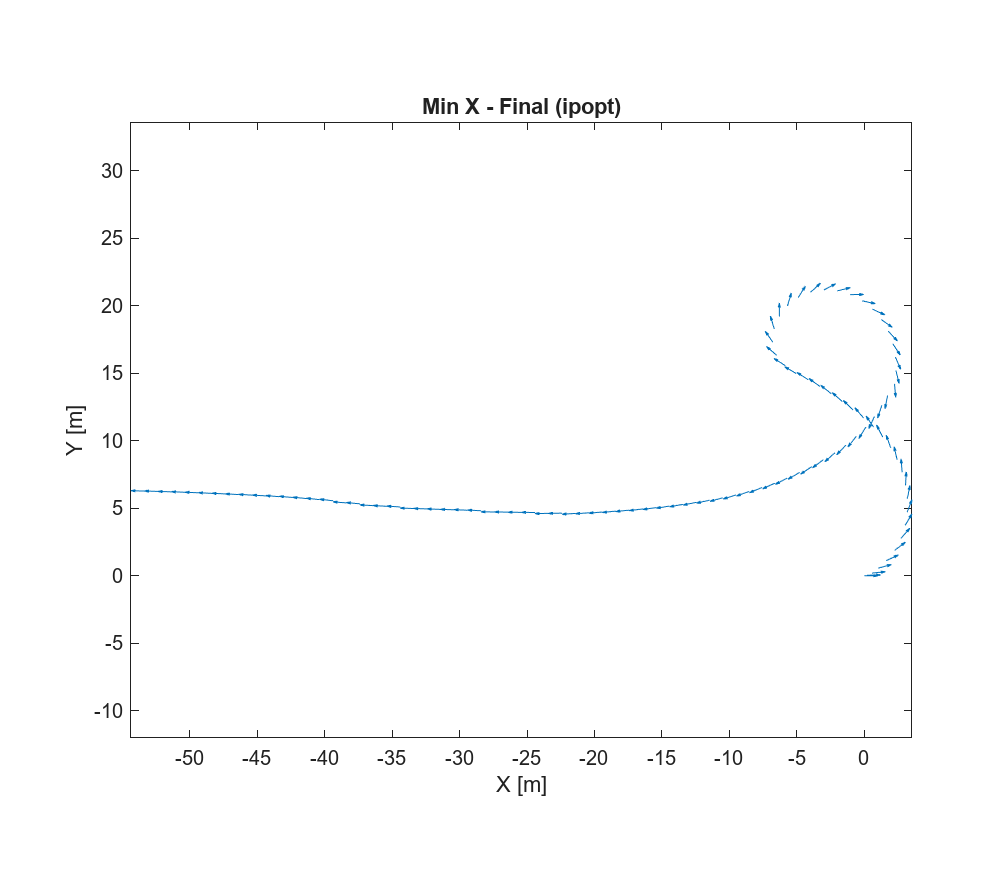
\includegraphics[width = \columnwidth]{figs/Min_X_-_Final_(ipopt)_quiver.png}
		\end{column}
		\begin{column}{0.4\textwidth}
			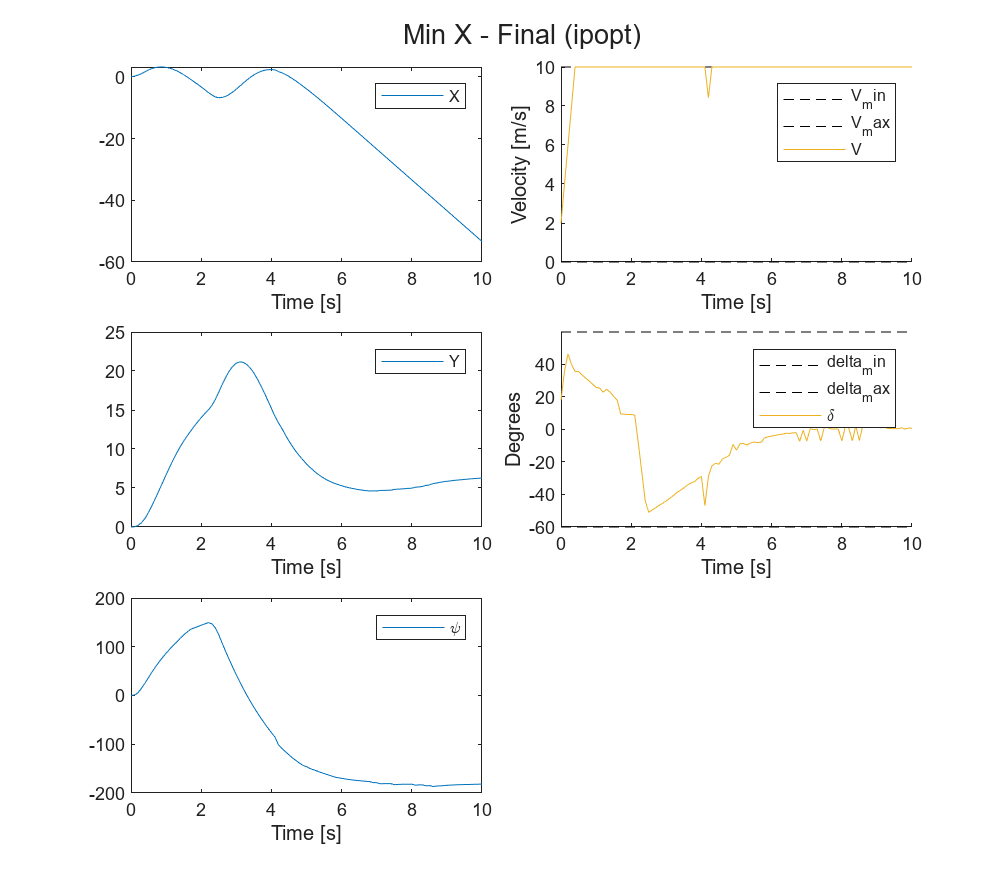
\includegraphics[width = \columnwidth]{figs/Min_X_-_Final_(ipopt)_traj.png}			
		\end{column}
	\end{columns}
\end{frame}


\begin{frame}
	\frametitle{fmincon vs ipopt (Min X w/ special ref - fmincon fails)}
	$J_k = x_k + (y_k - 0)^2/100 + (\theta_k - \pi)^2$
	\begin{columns}
		\begin{column}{0.4\textwidth}
			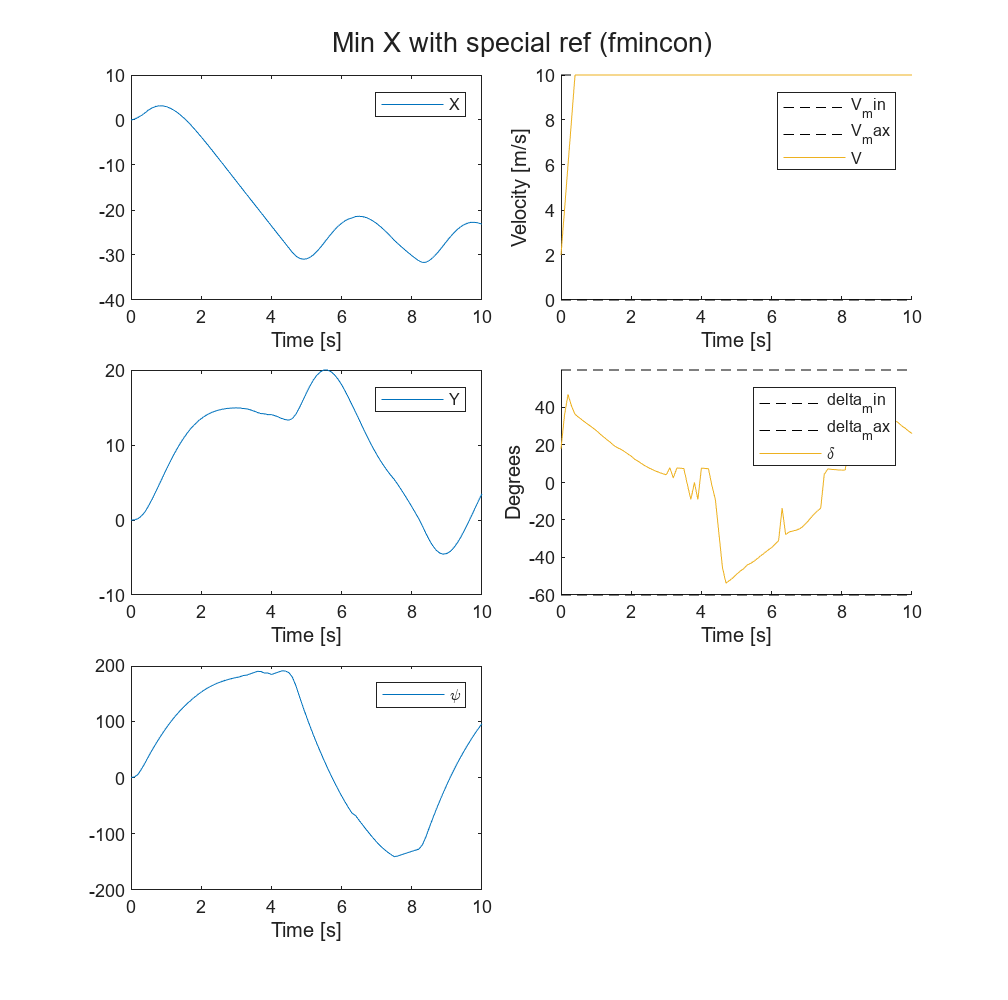
\includegraphics[width = \columnwidth]{figs/Min_X_with_special_ref_(fmincon)_traj.png}
		\end{column}
		\begin{column}{0.25\textwidth}
			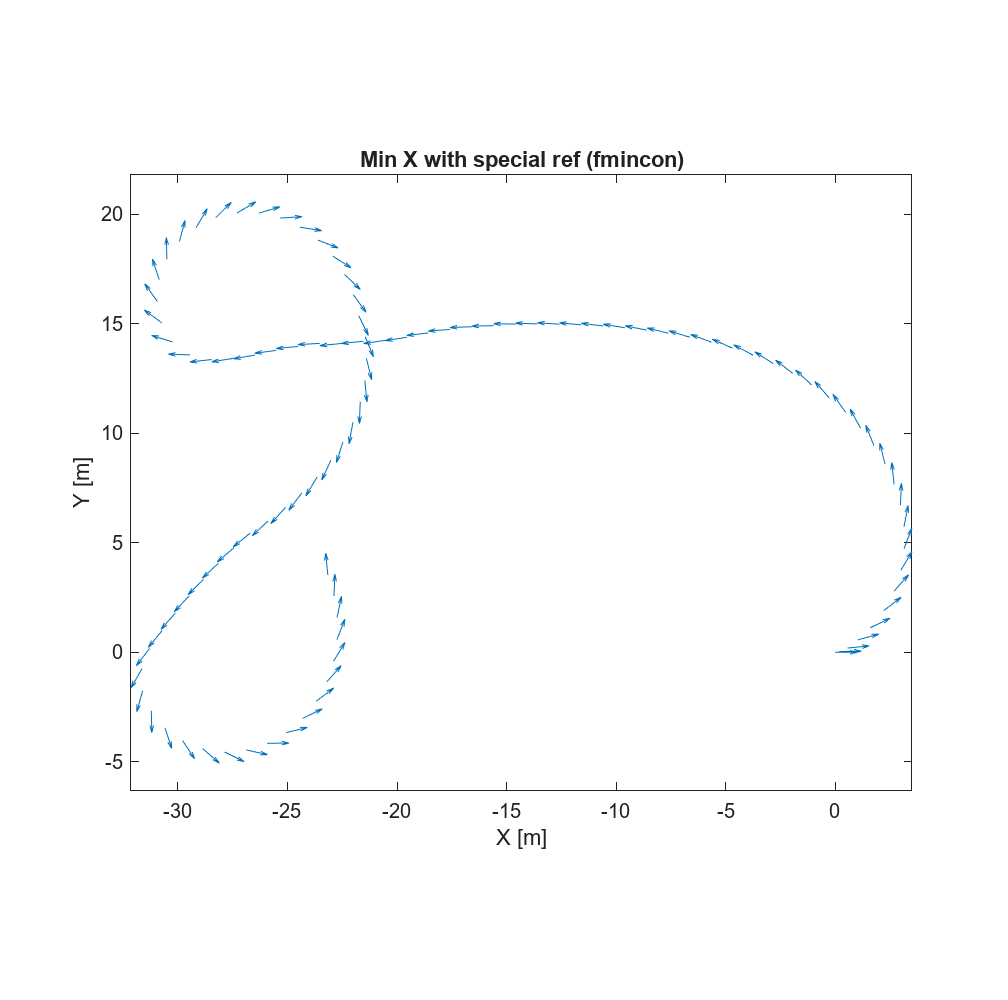
\includegraphics[width = \columnwidth]{figs/Min_X_with_special_ref_(fmincon)_quiver.png}
			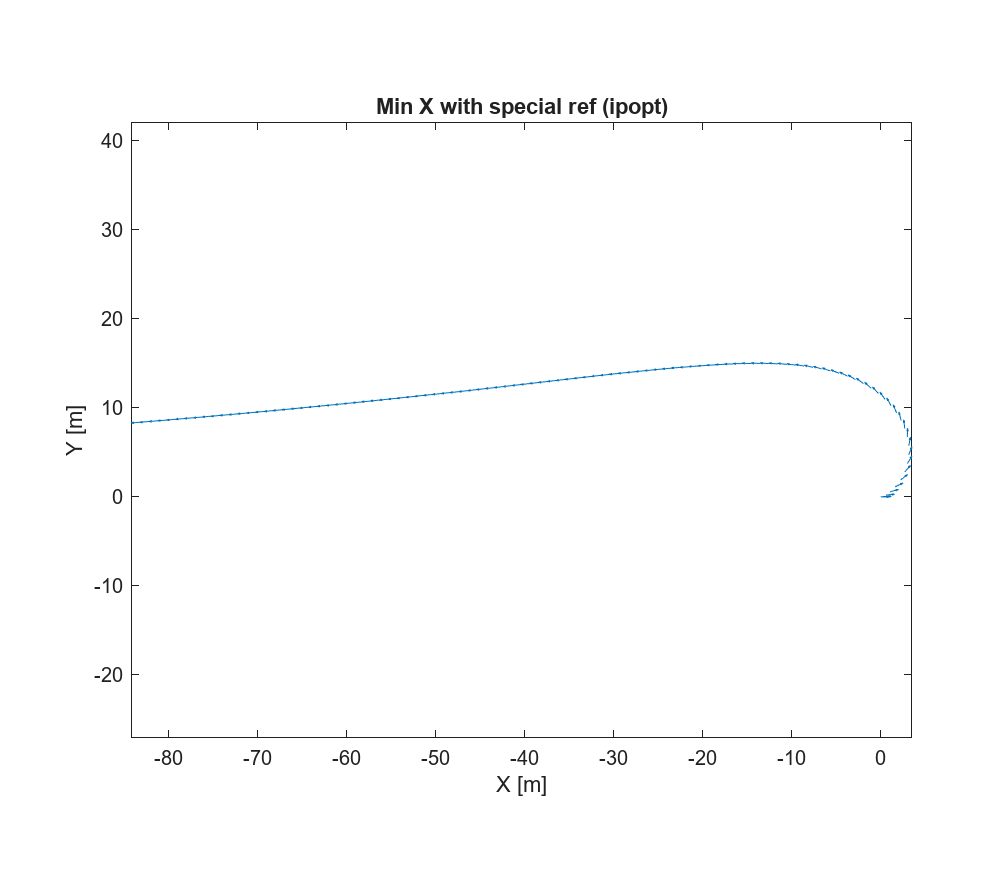
\includegraphics[width = \columnwidth]{figs/Min_X_with_special_ref_(ipopt)_quiver.png}
		\end{column}
		\begin{column}{0.4\textwidth}
			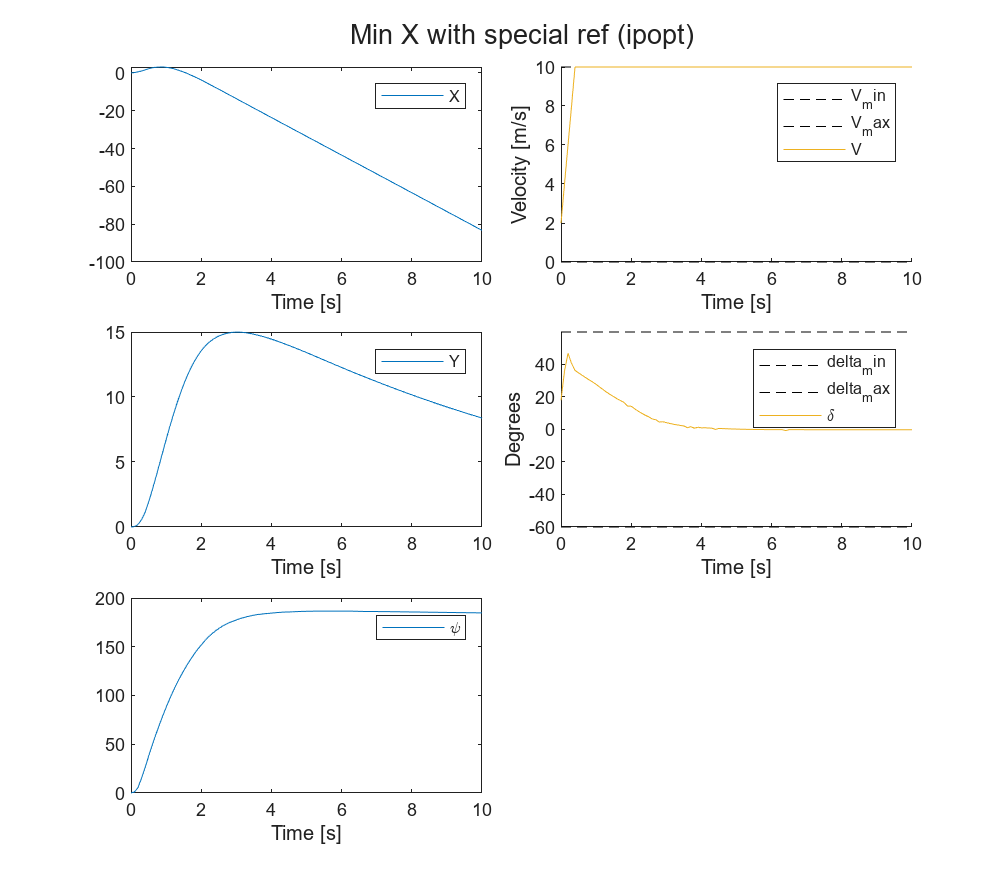
\includegraphics[width = \columnwidth]{figs/Min_X_with_special_ref_(ipopt)_traj.png}			
		\end{column}
	\end{columns}
\end{frame}


\begin{frame}
	\frametitle{fmincon vs ipopt (Max Y w/ Final - ipopt fails)}
	$J = -y_{N+1}$
	\begin{columns}
		\begin{column}{0.4\textwidth}
			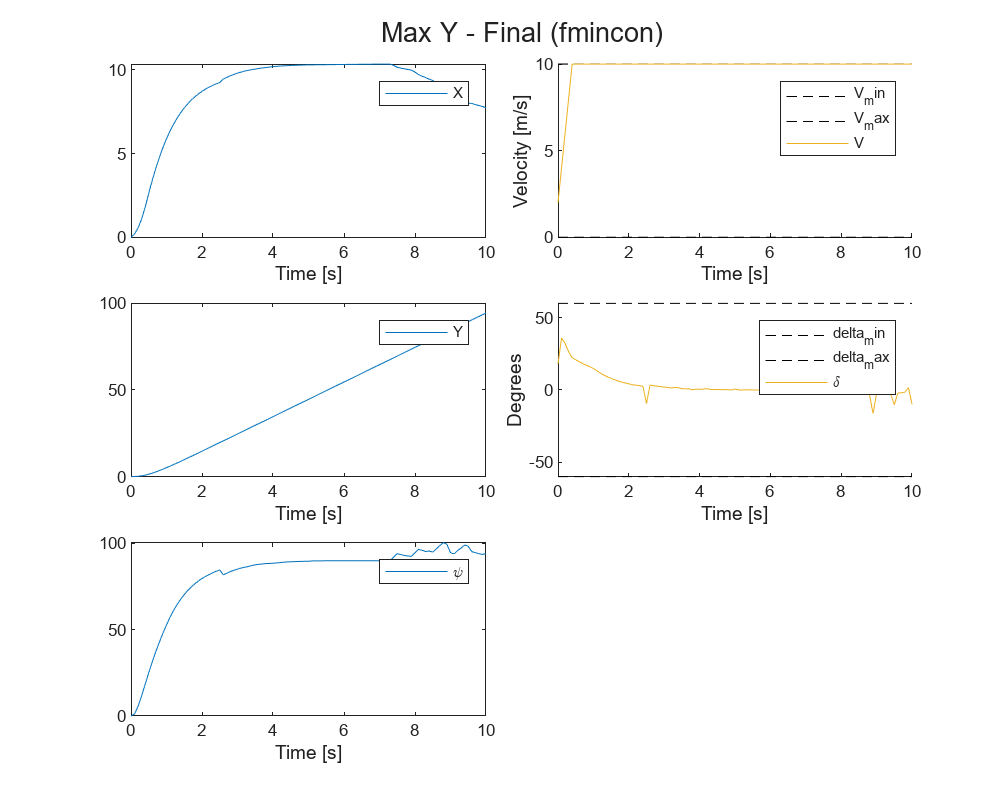
\includegraphics[width = \columnwidth]{figs/Max_Y_-_Final_(fmincon)_traj.png}
		\end{column}
		\begin{column}{0.25\textwidth}
			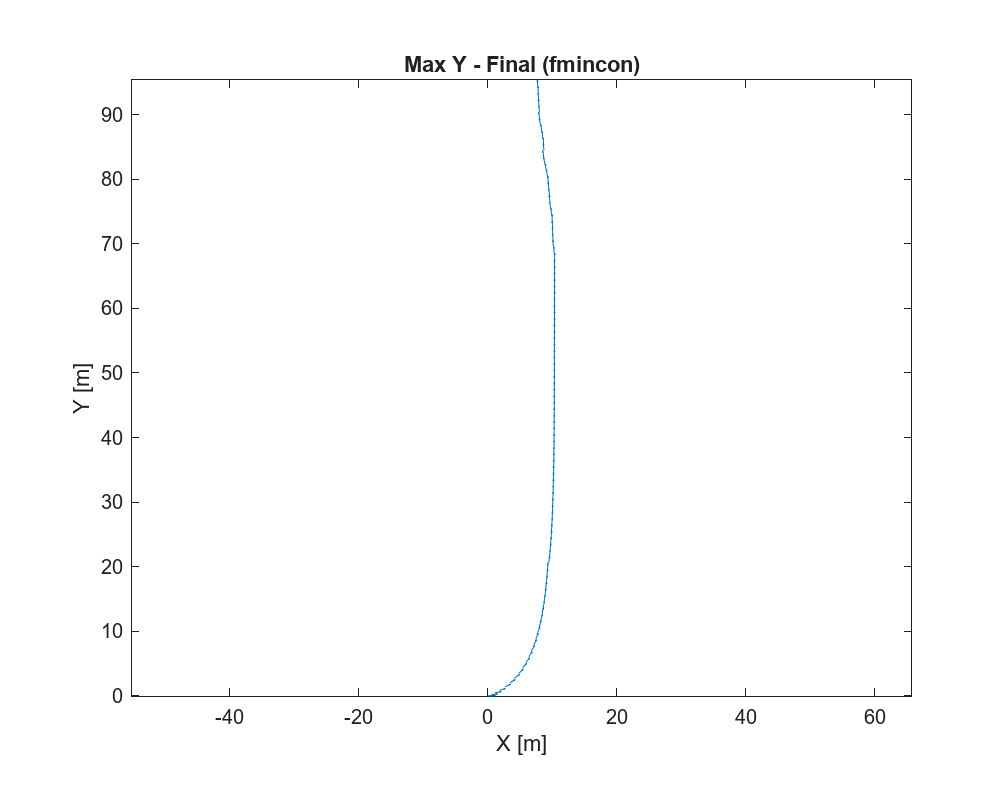
\includegraphics[width = \columnwidth]{figs/Max_Y_-_Final_(fmincon)_quiver.png}
			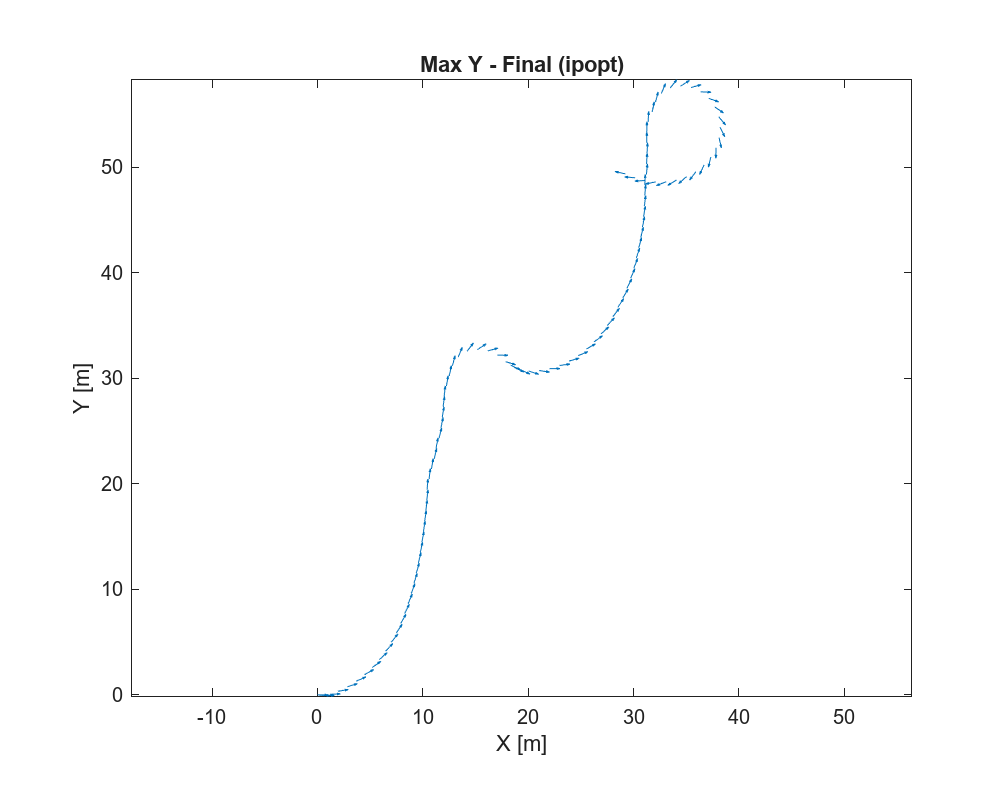
\includegraphics[width = \columnwidth]{figs/Max_Y_-_Final_(ipopt)_quiver.png}
		\end{column}
		\begin{column}{0.4\textwidth}
			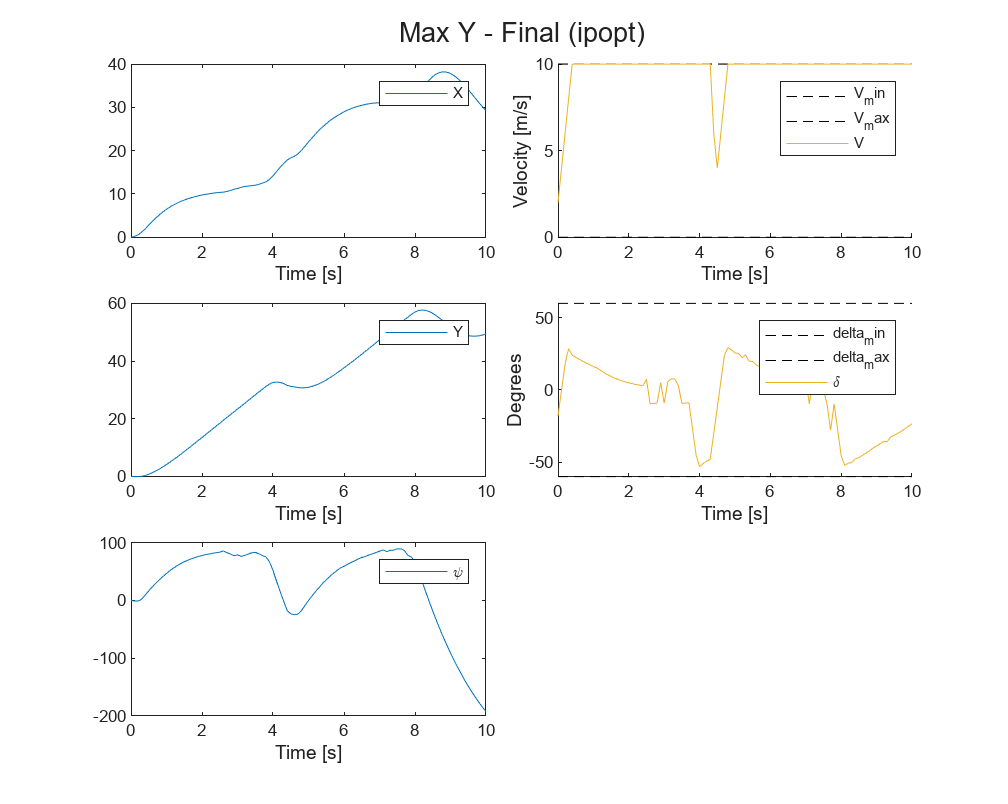
\includegraphics[width = \columnwidth]{figs/Max_Y_-_Final_(ipopt)_traj.png}			
		\end{column}
	\end{columns}
\end{frame}



\begin{frame}
	\frametitle{fmincon vs ipopt (Max Y with refs)}
	$J_k = -y_k + (x_k - 0)^2 + (\theta_k - \pi/2)^2$
	\begin{columns}
		\begin{column}{0.4\textwidth}
			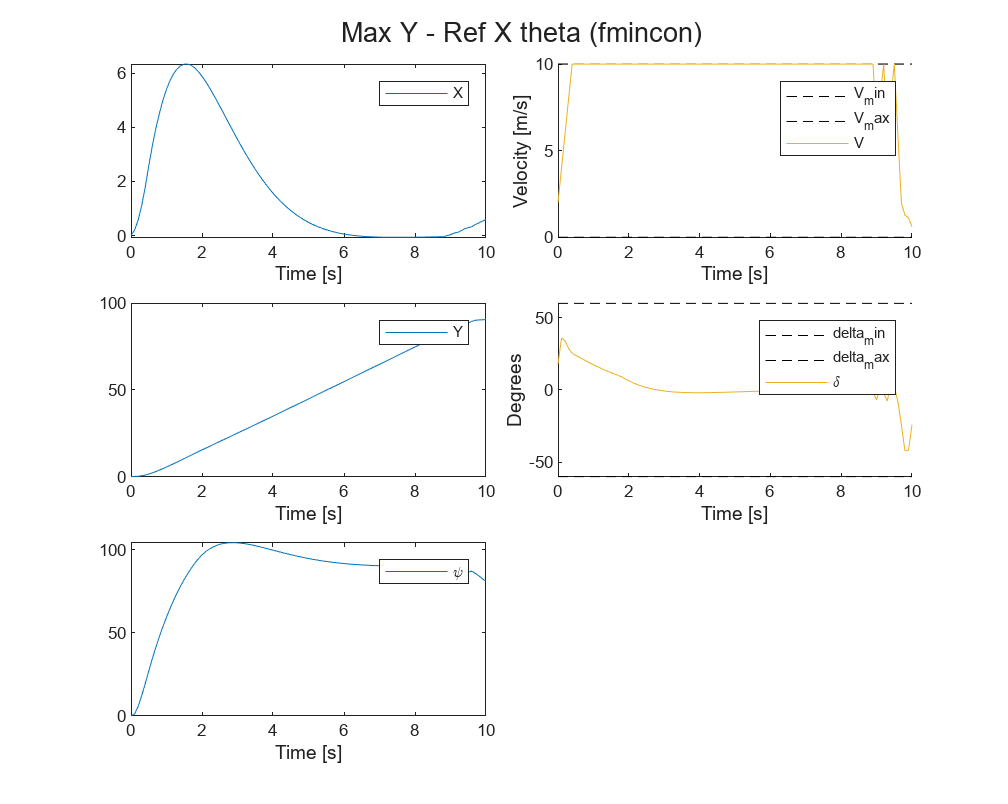
\includegraphics[width = \columnwidth]{figs/Max_Y_-_Ref_X_theta_(fmincon)_traj.png}
		\end{column}
		\begin{column}{0.25\textwidth}
			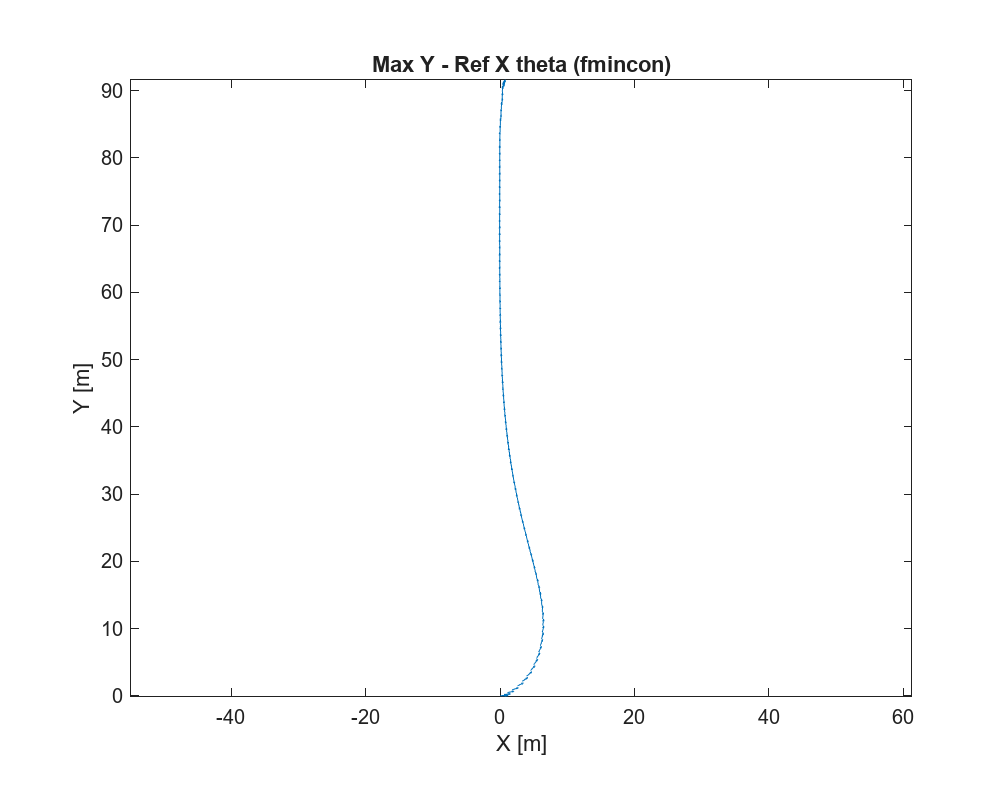
\includegraphics[width = \columnwidth]{figs/Max_Y_-_Ref_X_theta_(fmincon)_quiver.png}
			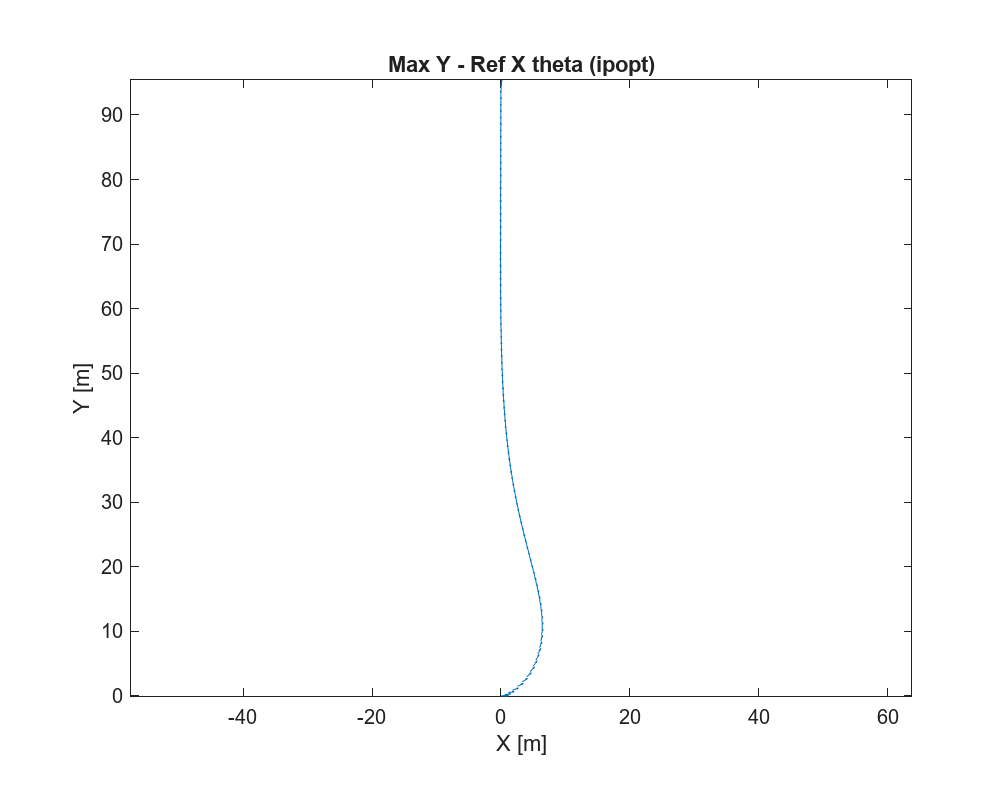
\includegraphics[width = \columnwidth]{figs/Max_Y_-_Ref_X_theta_(ipopt)_quiver.png}
		\end{column}
		\begin{column}{0.4\textwidth}
			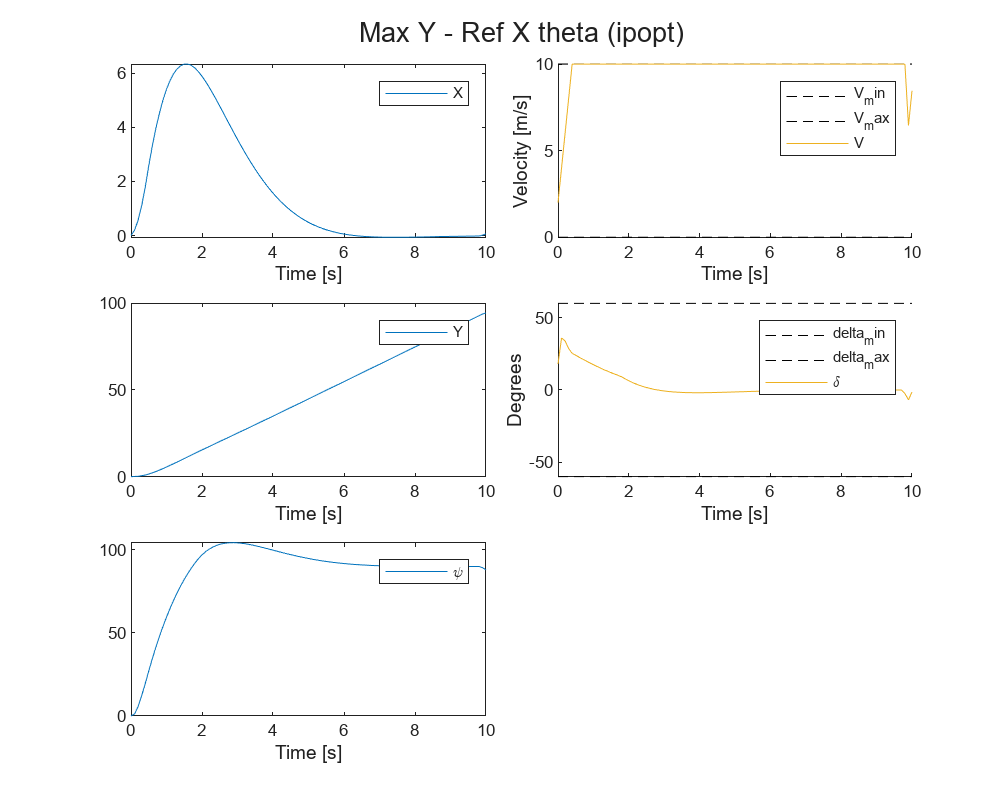
\includegraphics[width = \columnwidth]{figs/Max_Y_-_Ref_X_theta_(ipopt)_traj.png}			
		\end{column}
	\end{columns}
\end{frame}




% \subsection{Path Planning Implementation}
% \begin{frame}
% 	\frametitle{Path Planning Cost-Functions}
% 	The 
	

% \end{frame}



%% Final Section
\section*{}




\begin{frame}[allowframebreaks]{Bibliography}
	\bibliographystyle{unsrt}
	\bibliography{refs}
\end{frame}






\end{document}










% \section{Overview}

% \begin{frame}{Paper Information} %[t] places slide content at the top
%     \textbf{Title:} Kalman Filter Based Secure State Estimation and Individual Attacked Sensor Detection in Cyber-Physical Systems\\
%     \vspace{10 pt}
%     \textbf{Authors:} M. H. {Basiri} and J. G. {Thistle} and J. W. {Simpson-Porco} and S. {Fischmeister}\\
%     \vspace{10 pt}
%     \textbf{Conference:} 2019 American Control Conference (ACC)\\
%     \vspace{10 pt}
%     \textbf{Main Contributions:} Development and simulation of two attack detection and secure state estimation algorithms - Rolling Window Detector (RWD) and Novel Residual Detector (NRD)
% \end{frame}

% \begin{frame}{Security of Cyber-Physical Systems}
% 	\begin{itemize}
% 		\setlength \itemsep{1em}
% 		\item Cyber-Physical Systems (CPS) allow for large scale wide spread control systems that can take advantages of wireless data communication
% 		\item CPSs are unfortunately vulnerable to malicious attacks
% 		\item Attacks on a subset of sensors may attempt to disrupt the performance of such system
% 		\item Detection of such attacks is important and it is difficult to distinguish between noise and attacks
% 		\item Many detection methods actually use Kalmen filter estimation and perform hypothetical testing base the residual vector to detect changes above the standard noise threshold
% 	\end{itemize}
% \end{frame}

% \section{System and Attack Modeling}
% \begin{frame}{System and Attack Definitions}
% 	\begin{columns}
% 		\begin{column}{0.5\textwidth}
% 			\begin{center}
% 				\textbf{Original System}
% 			\end{center}
% 			\begin{equation}
% 				\mathcal{P}:
% 				\begin{cases}
% 					x_{k+1}=Ax_{k}+Bu_{k}+\nu_{k},\\
% 					 \quad y_{k}=Cx_{k}+w_{k}
% 				 \end{cases}
% 			\end{equation}\extraspace
% 			\textbf{States, Inputs, and Outputs:}\\
% 			$x\in \mathbb{R}^{n}$, $u\in \mathbb{R}^{m}$, and $y\in \mathbb{R}^{q}$\\ \extraspace
% 			\textbf{Noise:}
% 			$\nu\sim \mathcal{N}(0,\ Q)$ and $w\sim \mathcal{N}(0,R)$ \\ \extraspace
% 			\textbf{Initial State:}
% 			$x_0 \sim \mathcal{N}(0,\Sigma)$
% 		\end{column}
% 		\begin{column}{0.5\textwidth}
% 			\begin{center}
% 				\textbf{Attacked System}
% 			\end{center}
% 			\begin{equation}
% 				\mathcal{P}_{a}:
% 				\begin{cases}
% 					x_{k+1}^{a}=Ax_{k}^{a}+Bu_{k}+\nu_{k},\\
% 					 \quad y_{k}^{a}=Cx_{k}^{a}+w_{k}+Da_{k}
% 				 \end{cases}
% 			\end{equation}
% 			\textbf{States, Inputs, and Outputs:}
% 			$x_k^a$, $u_k$, and $y_k^a$\\ \extraspace
% 			\textbf{Noise:}
% 			$\nu\sim \mathcal{N}(0,\ Q)$ and $w\sim \mathcal{N}(0,R)$ \\ \extraspace
% 			\textbf{Attacks:}
% 			$a_k$ is manipulated\\ $D$ s.t. $D_{jj} = 1$ if $j^{th}$ sensor is under attack, otherwise $D_{ij} = 0 \ \forall i,j$
% 		\end{column}
% 	\end{columns}
% \end{frame}


% \section{Attack Detection Preliminaries}

% \subsection{Kalman Filtering}
% \begin{frame}{Kalman Filter Definition}
% 	\begin{columns}
% 		\begin{column}{0.5\textwidth}
% 			\centering
% 			\textbf{Measurement Update}
% 			\begin{align}
% 				K_{k}&=P_{k\vert k-1}C^{T}(CP_{k\vert k-1}C^{T}+R)^{-1}\\
% 				P_{k\vert k}&=P_{k\vert k-1}-K_{k}CP_{k\vert k-1}\\
% 				\hat{x}_{k\vert k}&=\hat{x}_{k\vert k-1}+K_{k}(y_{k}-C\hat{x}_{k\vert k-1})
% 			\end{align}
		
% 			\textbf{Time Update}
% 			\begin{align}
% 				&\hat{x}_{k+1\vert k}=A\hat{x}_{k\vert k}+Bu_{k}\\
% 				&P_{k+1\vert k}=AP_{k\vert k}A^{T}+Q
% 			\end{align}
			

% 		\end{column}
% 		\begin{column}{0.5\textwidth}
% 			\centering
% 			\textbf{Equivalent Equations:}
% 			\begin{align*}
% 				K_{k}&=P_{k}^{-} H^{T}(H P_{k}^{-} H^{T}+R)^{-1}\\
% 				P_{k}^{+} &= \qty(I - K_kH_k)P_{k}^{-}\\
% 				\hat{x}_{k}^{+} &= \hat{x}_{k}^{-} + K_{k}(y_{k}-H\hat{x}_{k}^{-})
% 			\end{align*}\\
% 			\begin{align*}
% 				&\hat{x}_{k}^{-} = F \hat{x}_{k-1}^{+} + G u_{k-1}\\
% 				&P_k^{-} = F P_{k-1}^{+} F^{T} + Q
% 			\end{align*}
% 		\end{column}
% 	\end{columns} \vskip 2em
% 			\textbf{Steady-State:}  $
% 				P\mathop{=}^{\triangle} \lim_{k\rightarrow\infty}P_{k\vert k-1}$
% 				\hspace{1em}
% 				$K \mathop{=}^{\triangle} \lim_{k\rightarrow\infty} K_{k}=PC^{T}(CPC^{T}+R)^{-}$

% \end{frame}

% \subsection{Conventional $\chi^2$-Detector}
% \begin{frame}{Conventional $\chi^2$-Detector}
% 	\begin{flushleft}
% 		Widely used in fault-detection and also applicable to CPS security.
% 	\end{flushleft}
% 	\begin{columns}
% 		\begin{column}{0.5\textwidth}
% 			\textbf{Residual Vector:}
% 			\begin{equation}
% 				r_k = y_k - \hat{y}_k = y_k - C \hat{x}_k
% 			\end{equation}
% 			\textbf{Residual Covariance:}
% 			\begin{equation}
% 				\Sigma_{r,k} = C {k \vert k} C^{T} + R
% 			\end{equation}
% 			\textbf{Residual Power:}
% 			\begin{equation}
% 				g_k = r_k^T \Sigma_{r,k}^{-1} r_k
% 			\end{equation}
% 		\end{column}
% 		\begin{column}{0.05\textwidth}\end{column}
% 		\begin{column}{0.45\textwidth}
% 			\textbf{Detector Statistical Test:}\\
% 			A threshold determined using the desired confidence and degrees of freedom from the $chi^2$-distribution. An alarm is then triggered if:
% 			\begin{equation}
% 				g_k > threshold
% 			\end{equation}
% 			\vspace{2em}
% 		\end{column}
% 	\end{columns}
% \end{frame}


% \section{Proposed Attack Detection Algorithms}

% \subsection{RWD Attack Detector}
% \begin{frame}{Rolling Window Detector (RWD)}
% 	\begin{columns}
% 		\begin{column}{0.5\textwidth}
% 			This detector works by comparing the measured residual cumulative sum $\bar{P}_{k \vert k}$ over a set period of time $T$ with the error covariance predicted by the Kalman filter, $P_{k \vert k}$.\\ \extraspace
% 			\textbf{Test Definitions:}
% 			\begin{align}
% 				\hat{\Sigma}_k &= \frac{1}{T} \sum_{k=k_0}^{k_0 + T -1} (y_k-\hat{y}_k)(y_k-\hat{y}_k)^{T}\\
% 				\Sigma_{r,k} &= C P_{k \vert k} C^{T} + R
% 			\end{align}
% 			\textbf{Testing Statistic:} ($H$ is the threshold matrix)
% 			\begin{equation}
% 				S(T,k_0) = \hat{\Sigma}_k - \Sigma_{r,k} > H
% 			\end{equation}
% 		\end{column}
% 		\begin{column}{0.05\textwidth}\end{column}
% 		\begin{column}{0.45\textwidth}
% 			\includegraphics[width=\columnwidth]{figs/RWD_Procedure}
% 		\end{column}
% 	\end{columns}
% \end{frame}

% \begin{frame}{RWD Procedure}
% 	\begin{columns}
% 		\begin{column}{0.33\textwidth}
% 			\includegraphics[width=\columnwidth]{figs/RWD_Diagram}
% 		\end{column}
% 		\begin{column}{0.05\textwidth}\end{column}
% 		\begin{column}{0.5\textwidth}
% 			\includegraphics[width=\columnwidth]{figs/RWD_Procedure}
% 		\end{column}
% 	\end{columns}
% \end{frame}

% \subsection{NRD Attack Detector}
% \begin{frame}{Novel Residual Detector (NRD)}
% 	\begin{columns}
% 		\begin{column}{0.5\textwidth}
% 			This method extends the $\chi^2$-detector method to individual sensors using a similar modified Kalman filter to RWD.\\ \extraspace
% 			\textbf{Test Definitions:} (First is identical to $\chi^2$-test)
% 			\begin{align}
% 				g_k &= r_k^T \Sigma_{r,k}^{-1} r_k > threshold_1\\
% 				g_{j,k} &= \frac{r_k^2}{(\Sigma_{r,k})_jj} > threshold_2
% 			\end{align}
% 		\end{column}
% 		\begin{column}{0.05\textwidth}\end{column}
% 		\begin{column}{0.45\textwidth}
% 			\includegraphics[width=\columnwidth]{figs/NRD_Procedure}
% 		\end{column}
% 	\end{columns}
% \end{frame}

% \begin{frame}{NRD Procedure}
% 	\begin{columns}
% 		\begin{column}{0.35\textwidth}
% 			\includegraphics[width=\columnwidth]{figs/NRD_Diagram}
% 		\end{column}
% 		\begin{column}{0.05\textwidth}\end{column}
% 		\begin{column}{0.45\textwidth}
% 			\includegraphics[width=\columnwidth]{figs/NRD_Procedure}
% 		\end{column}
% 	\end{columns}
% \end{frame}


% \section{Simulation Result}
% \begin{frame}{IEEE 14-bus Power Grid System \cite{CyberPhysicalAttacksOnPowerNetworks}}
% 	\begin{columns}
% 		\begin{column}{0.55\textwidth}
% 			Effectiveness of RWD and NRD is tested on the IEEE 14-bus power grid system
% 			\begin{itemize}
% 				\item 5 generators and 14 buses
% 				\item 14 power injection and 20 power flow sensors
% 			\end{itemize}
% 			\textbf{System Parameters:} $n = 10$ and $p = 35$\\
% 			\textbf{System States:}\\ $\delta_i$ (rotor angle), $\omega_i$ (frequencies) $\forall \ i = \{1,\cdots, \frac{n}{2}\}$
% 		\end{column}
% 		\begin{column}{0.45\textwidth}
% 			\includegraphics[width=\columnwidth]{figs/Simulation_Power_Grid}
% 		\end{column}
% 	\end{columns}
% \end{frame}
% \begin{frame}{Simulation Results Overview}
% 	The simulation tested the two methods for 3 cases:
% 	\begin{itemize}
% 		\item The Unstealthy Case - Attempts to disrupt system without remaining undetected
% 		\item The Stealthy Case - Injects false data upon the same order as the noise
% 		\item The Very Unstealthy Case - An unstealthy attack much larger then the noise
% 	\end{itemize}
% 	\centering
% 	\includegraphics[width=0.7\textwidth]{figs/Sim_Measurment_Comparrision}
% \end{frame}


% \subsection{The Unstealthy Case}
% \begin{frame}{The Unstealthy Case}
% 	\centering
% 	\includegraphics[width=0.9\textwidth]{figs/Sim_Error_Comparrision_Unstealthy}\\
	
% 	Estimation error compared with the {Imhotep-SMT tool \cite{Imhotep_SMT}} and a standard Kalman Filter.
% \end{frame}

% \begin{frame}{The Unstealthy Case - Individual Sensors}
% 	\centering
% 	\includegraphics[width=0.6\textwidth]{figs/Sim_Error_Sensors}\\
	
% 	Residuals calculated for individual sensors for RWD and NRD (unstealthy attacks).
% \end{frame}


% \subsection{The Stealthy Case}
% \begin{frame}{The Stealthy Case}
% 	\centering
% 	\includegraphics[width=0.9\textwidth]{figs/Sim_Error_Comparrision_Stealthy}\\
% 	Estimation error compared with the {Imhotep-SMT tool \cite{Imhotep_SMT}} and a standard Kalman Filter.
% \end{frame}

% \subsection{The Very Unstealthy Case}
% \begin{frame}{The Very Unstealthy Case}
% 	\centering
% 	\includegraphics[width=0.9\textwidth]{figs/Sim_Error_Comparison_VeryUnstealthy}\\
% 	Estimation error compared with the {Imhotep-SMT tool \cite{Imhotep_SMT}} and a standard Kalman Filter.
% \end{frame}

% \begin{frame}{The Very Unstealthy Case - Individual Sensor}
% 	\centering
% 	\includegraphics[width=0.9\textwidth]{figs/Sim_StateEstimation_VeryUnstealthy}\\
	
% 	Estimation error of state $x_7$ for RWD and NRD (very unstealthy attacks).
% \end{frame}

% \subsection{Detection Rate Analysis}
% \begin{frame}{Detection Rate Analysis}
% 	\textbf{False Positive Rate (FPR):} $FNR = \frac{FN}{FP + TP}$
	
% 	\centering
% 	\includegraphics[width=0.7\textwidth]{figs/Sim_FNR_SMPvsNRD}\\
% 	FNR for Imhotep-SMT vs NRD. NRD clearly performs better then Imhotep-SMT when the attack and noise power decrease (aka stealthy case).

% \end{frame}

% \section*{}
% \begin{frame}{Questions?}
% 	\begin{columns}
% 		\begin{column}{0.3\textwidth}
% 			\centering
% 			\includegraphics[width=\columnwidth]{figs/Simulation_Power_Grid}
% 			\includegraphics[width=0.8\columnwidth]{figs/Sim_Error_Sensors}
% 		\end{column}
% 		\begin{column}{0.35\textwidth}
% 			\includegraphics[width=\columnwidth]{figs/Sim_Error_Comparrision_Unstealthy}
% 			\includegraphics[width=\columnwidth]{figs/Sim_Error_Comparrision_Stealthy}
% 			\includegraphics[width=\columnwidth]{figs/Sim_Error_Comparison_VeryUnstealthy}
% 		\end{column}
% 		\begin{column}{0.25\textwidth}
% 			\includegraphics[width=\columnwidth]{figs/Sim_FNR_SMPvsNRD5}
% 		\end{column}
% 	\end{columns}
% \end{frame}



% \begin{frame}[allowframebreaks]{Bibliography}
% 	\bibliographystyle{unsrt}
% 	\bibliography{mybib}
% \end{frame}




%\section[MLS Model]{Magnetic Levitation System Model}
%
%%\begin{frame}{Apparatus and Nonlinear Model}
%%    \begin{columns}
%%        \begin{column}{.6\textwidth}
%%            \begin{itemize}
%%                \item The MLS system is an inherently nonlinear and unstable system 
%%                \item An advantage of the MLS system is their is no friction and noise  
%%                \item These advantages can be explored in many applications such as 
%%                    MagLev Trains, Magnetic Bearings, and conveyor system
%%            \end{itemize}
%%        \end{column}
%%        \begin{column}{.4\textwidth}
%%            \includegraphics[width=\columnwidth]{figs/MLS_Diagram.PNG}\\
%%            \footnotesize{Diagram of Magnetic Levitation System}
%%        \end{column}
%%    \end{columns}
%%    
%%    
%%\end{frame}
%
%% \begin{frame}{Apparatus and Nonlinear Model}{Other Approaches}
%%     \begin{itemize}
%%         \item References to other proposed techniques to improve control in MLS-base applications
%%             \begin{itemize}
%%                 \item 
%%             \end{itemize}
%%     \end{itemize}
%% \end{frame}
%
%
%
%\begin{frame}[allowframebreaks]{MLS Model Linearization}
%	The MLS model was linearized using a series expansion method\\
%	\vspace{10pt}
%	\begin{align}
%		\intertext{\textbf{Nonlinear Model:}}
%		m\ddot{x}   &= mg-k \frac{i^2}{x^2}, \ i=k_1u\\
%		\ddot{x}    &= g - f(x,i), \ f(x,i) = \frac{ki^2}{mx^2}\\
%		\intertext{\textbf{Nonlinear Series Expansion} \newline 
%			With $\ddot{x}=0$, linearization is done about the equilibrium points: $x_0=-1.5 \ [V], \ i_0=0.8 \ [A]$}
%		\Ddot{x}    &=-\qty(\pdv{f(i,x)}{i}\eval_{i_0,x_0}\Delta i+\pdv{f(i,x)}{x}\eval_{i_0,x_0}\Delta x)\\
%		\intertext{\textbf{Linearized Transfer Function}}
%		\frac{\Delta X(s)}{\Delta I(s)} &=\frac{-K_i}{s^2+K_x}, \ \ \ K_i = \frac{2mg}{i_0} \ \text{and} \ K_x = \frac{2mg}{x_0} 
%	\end{align}
%	System transfer function is verified with a system identification procedure
%\end{frame}
%
%\section[Digital FO-PID Controller Design]{Design of a Digital Fractional Order PID Controller}
%
%\begin{frame}{Fractional Calculus}
%	`    \begin{columns}
%		\begin{column}{.5\columnwidth}
%			\textbf{Definition of a Diff-Integral}
%			\begin{displaymath}
%				D^\alpha = 
%				\begin{cases}
%					\dv[\alpha]{t}                  & \alpha > 0\\
%					1                               & \alpha = 0\\
%					\int_a^t (\dd \tau)^{-\alpha}   & \alpha < 0\\
%				\end{cases}
%			\end{displaymath}
%			\textbf{Riemann-Liousville (RL) Definition:}
%			\begin{align*}
%				_a D_t^\alpha f(t) = \frac{1}{\Gamma(n-\alpha)} \qty(\dv{t})^n \int_a^t \frac{f(\tau)}{(t-\tau)^{\alpha-n+1}} \dd \tau\\
%				\mathcal{L} \qty{_a D_t^\alpha f(t)} = s^{\pm \alpha} F(s)
%			\end{align*}
%		\end{column}
%		\begin{column}{.5\textwidth}
%			\textbf{Grunewald-Letnikov (GL) Definition:}
%			\begin{displaymath}
%				_a D_t^\alpha f(t) = \lim_{h\rightarrow 0} h^{-\alpha} \sum_{j=0}^{\qty[\frac{t-\alpha}{h}]} (-1)^j \mqty(\alpha\\ j) f(t-jh)
%			\end{displaymath}
%			\textbf{Caputo Fractional Derivative Definition:}
%			\begin{displaymath}
%				_a^C D_t^\alpha f(t) = \frac{1}{\Gamma(n-\alpha)} \int_a^t \frac{f^n(\tau)}{(t-\tau)^{\alpha-n+1}} \dd \tau
%			\end{displaymath}
%		\end{column}
%		
%	\end{columns}
%	\vspace{15pt}
%\end{frame}
%
%%\begin{frame}{Compensator Design}
%%    \textbf{Compensator Objective:} Shift the frequency response to a phase of $-36^\circ \pm 1\%$ \\
%%    \vspace{10pt}
%%    \textbf{Why?} Matching the frequency response of a fractional order integrator $(\alpha=-0.4)$\\
%%    \vspace{10pt}
%%    \textbf{Method:}
%%    Poles and Zeros are selected to maintain the phase value, $\phi_{req}$ within a tolerance, for a specific frequency band, $\omega_l \leq \omega \leq \omega_h$:
%%    \begin{columns}
%%        \begin{column}{.35\textwidth}
%%            \begin{align*}
%%                p_1 &= 10^{\qty[\frac{\phi_{req} + 45 \omega_l}{45}+1]}\\
%%                z_1 &= 10\omega_l\\
%%                p_2 &= 10^{\qty[{\log(p_1)+2-\mu}]}\\
%%                z_2 &= 10^{\qty[{\log(z_1)+2-\mu}]}\\
%%                    &\vdots\\
%%                p_n &\geq \omega_h
%%            \end{align*}
%%        \end{column}
%%        \begin{column}{.5\textwidth}
%%            \includegraphics[width=\columnwidth]{figs/AsymptoticPhasePlot.PNG}
%%        \end{column}
%%        \begin{column}{.05\columnwidth}
%%        \end{column}
%%    \end{columns}
%%\end{frame}
%%
%%\begin{frame}{Discretizing Fractional Order Integrator}
%%    \begin{columns}
%%        \begin{column}{.5 \textwidth}
%%            \begin{itemize}
%%                \item Multiple approximation methods were tested to discritize the system
%%                \item The Tustin approximation method was chosen with a sample time of .01 s
%%            \end{itemize}
%%            \begin{align*}
%%                z=e^{sT_s}\approx\frac{1+\frac{sT_s}{2}}{1-\frac{sT_s}{2}}
%%            \end{align*}
%%
%%        \end{column}
%%        \begin{column}{.5 \textwidth}
%%            \centering
%%             Approximation Method Comparison
%%            \includegraphics[width=.9\columnwidth]{figs/ApproxMethods.PNG}
%%            \vspace{5pt}
%%        \end{column}
%%    \end{columns}
%%    \centering
%%    
%%    $\begin{array}{|c|c c c c c c c |}
%%        \hline
%%        i   & 1     & 2     & 3     & 4     & 5     & 6     & 7\\
%%        \hline
%%        z_i & -0.9253   & -0.4842   & 0.9307    & 0.9920    & 0.9991    & 1     & 0.5136\\
%%        p_i & -0.8286   & 0.7651    & 0.9707    & 0.9767    & 1         & 1     & -0.0875\\
%%        \hline
%%    \end{array}$\\
%%    Pole-Zero Pairs of approximation for $s^{-0.4}$ with $0.1 \leq \omega \leq 100$ [rad/s]
%%\end{frame}
%%
%%\begin{frame}{Fractional Order Integrator Realization in MATLAB}
%%    \begin{columns}
%%        \begin{column}{.6\textwidth}
%%            \begin{itemize}
%%                \item MATLAB was used to recreate an digital approximation for the fractional order integrator
%%                \item The resulting bode plot demonstrates that the compensator designed with the procedure described did not meet specifications
%%                \item The pole-zero values provided directly in the paper were also tested and did not meet specifications either
%%            \end{itemize}
%%        \end{column}
%%        \begin{column}{.4\textwidth}
%%            \includegraphics[width=\columnwidth]{figs/BodeSim.png}
%%        \end{column}
%%    \end{columns}
%%\end{frame}
%%
%%
%%
%%\begin{frame}{Digital FO-PID Controller}
%%    \begin{columns}
%%        \begin{column}{.4 \textwidth}            
%%        $\begin{array}{|c | c c c c c |}
%%            \hline
%%            \text{Controller}   & K_p   & K_i   & K_d   & \alpha    & \beta\\
%%            \hline
%%            \text{PD}           & 4     & -     & 2     & -         & 1 \\
%%            \text{PID}          & 5.5   & 2     & 0.2   & 1         & 1 \\
%%            \text{FO-PID}       & 7     & 12    & 1     & 0.4       & 0.8 \\
%%            \hline
%%        \end{array}$
%%        \tiny{Parameters were optimized using Dynamic Particle Swarm Optimization (dPSO)}
%%        \end{column}
%%        \begin{column}{.6 \textwidth}
%%            \includegraphics[width=\columnwidth]{figs/DigitalFO-PIDBlockDiagram.PNG}
%%
%%        \end{column}
%%    \end{columns}
%%\end{frame}
%%
%%\section{Compensator Simulation and Testing Results}
%%
%%\begin{frame}{Simulation Results}
%%    \begin{columns}
%%        \begin{column}{.6\textwidth}
%%            \begin{itemize}
%%                \item Displays the simulation results, done using MATLAB
%%                \item The amount of deviation decreases when the complexity of the compensator is increased
%%            \end{itemize}
%%            \setstretch{2}
%%            \tiny{
%%            $\begin{array}{|c | c c c c | }
%%                  \hline
%%                  \text{Ball Position(m)} & & \text{PD} & \text{PID} & \text{FO-PID}\\
%%                  \hline                  
%%                  &  \text {Max} & 8.12 \cross 10^{-3} &6.92 \cross 10^{-3} & 5.94 \cross 10^{-3}\\
%%                  \text{Measured} & \text{Min} & -4.83 \cross 10^{-3} & -6.68 \cross 10^{-3} & -5.65 \cross 10^{-3}\\
%%                  \hline
%%                  & \text{Max}&5.5 \cross 10^{-3} &5.5 \cross 10^{-3} & 5.5 \cross 10^{-3}\\
%%                  \text{Desired} & \text{Min}&-5.5\cross 10^{-3} & -5.5\cross 10^{-3} & -5.5\cross 10^{-3}\\
%%                  \hline
%%                  \text{Error} & & 23.06\% &19.09\% & 5.03\% \\
%%                  \hline
%%            \end{array}$
%%            }
%%            \setstretch{1}
%%        \end{column}
%%        \begin{column}{.35\textwidth}
%%            \includegraphics[width=\columnwidth]{figs/SimResults_PD.PNG}\\
%%            \includegraphics[width=\columnwidth]{figs/SimResults_PID.PNG}\\
%%            \includegraphics[width=\columnwidth]{figs/SimResults_FO-PID.PNG}\\
%%            \tiny{Simulation results of PD (top), PID (middle), and FO-PID (bottom) controllers}
%%        \end{column}
%%        \begin{column}{.05\textwidth}
%%        \end{column}
%%    \end{columns}    
%%\end{frame}
%%
%%\begin{frame}{Real-time Test Results}
%%    \begin{columns}
%%        \begin{column}{.5\textwidth}
%%            \setstretch{2}
%%            \tiny{
%%            $\begin{array}{|c | c c c c | }
%%                  \hline
%%                  \text{Ball positions (m)} & & \text{PD} & \text{PID} & \text{FO-PID}\\
%%                  \hline                  
%%                  &  \text {Max} & 16.8\cross 10^{-3} & 13.1\cross 10^{-3} & 12.6\cross 10^{-3}\\
%%                  \text{Measured} & \text{Min} & 8.3\cross 10^{-3}&4.85\cross 10^{-3} & 5.24\cross 10^{-3}\\
%%                  \hline
%%                  & \text{Max}&12.5\cross 10^{-3}&12.5\cross 10^{-3} & 12.5\cross 10^{-3}\\
%%                  \text{Desired} & \text{Min}&5.5\cross 10^{-3} & 5.5\cross 10^{-3} & 5.5\cross 10^{-3}\\
%%                  \hline
%%                  \text{Error} & & 29.66\% & 8.95\% & 5.75\% \\
%%                  \hline
%%            \end{array}$
%%            }
%%            \setstretch{1}
%%        \end{column}
%%        \begin{column}{.4\textwidth}
%%            \includegraphics[width=\columnwidth]{figs/TestResults_PD.PNG}\\
%%            \includegraphics[width=\columnwidth]{figs/TestResults_PID.PNG}\\
%%            \includegraphics[width=\columnwidth]{figs/TestResults_FO-PID.PNG}\\
%%            \tiny{Real-time test results of PD (top), PID (middle), and FO-PID (bottom) controllers}
%%        \end{column}
%%        \begin{column}{.05\textwidth}
%%        \end{column}
%%    \end{columns}    
%%\end{frame}
%%
%%
%%\begin{frame}{Control Effort Comparison}
%%    \begin{columns}
%%        \begin{column}{.5\textwidth}
%%            \setstretch{1.5}
%%            \tiny{
%%            $\begin{array}{|c | c c c c | }
%%                  \hline
%%                  \text{Performance indices} & & \text{PD} & \text{PID} & \text{FO-PID}\\
%%                  \hline                  
%%                  &  \text {Error signal} & 51.97 & 14.56 & 12.79\\
%%                  \text{IAE} & \text{Control signal} & 208 & 181 & 151.5\\
%%                  \hline
%%                  & \text{Error signal}&609 &455.7 & 425.5\\
%%                  \text{ITAE} & \text{Control signal}&900.6 & 797.9 & 602.5\\
%%                  \hline
%%                  & \text{Errorsignal} & 28.38 & 4.978 & 2.488\\
%%                  \text{ISE} & \text{Control signal}& 832.6 & 647.2 & 347.2 \\
%%                  \hline
%%            \end{array}$
%%            }
%%            \setstretch{1}
%%        \end{column}
%%        \begin{column}{.4\textwidth}
%%            \includegraphics[width=\columnwidth]{figs/ControlEffortAnalysis.PNG}\\
%%            \tiny{Comparison of Control Effort Between Controllers}
%%        \end{column}
%%        \begin{column}{.05\textwidth}
%%        \end{column}
%%    \end{columns}    
%%\end{frame}
%%
%%
%%
%%\begin{frame}{Conclusion}
%%    \begin{columns}
%%        \begin{column}{.3\textwidth}
%%        \includegraphics[width=\columnwidth]{figs/MLS_Diagram.PNG}
%%        \includegraphics[width=\columnwidth]{figs/ControlEffortAnalysis.PNG}
%%
%%        \end{column}
%%        \begin{column}{.4\textwidth}
%%        \includegraphics[width=\columnwidth]{figs/DigitalFO-PIDBlockDiagram.PNG}
%%        \end{column}
%%    \end{columns}
%%\end{frame}